% This is samplepaper.tex, a sample chapter demonstrating the
% LLNCS macro package for Springer Computer Science proceedings;
% Version 2.21 of 2022/01/12


% TODOs:
% 1) Check what's needed and add the annexes
% 2) Finir de transferer les annexes mais pluot filtrer a la lecture du manuscrit 
% 3) Compresser par lecture (ipad serait pas mal) 
% 4) Update certaines parties notmment avec de la literature 
% 5) Voir les derniers articles de la conf ? 
% 6) Update experiments ? 

% Check the MAYBE, 

%
\documentclass[runningheads]{llncs}
%


\usepackage[T1]{fontenc}
% T1 fonts will be used to generate the final print and online PDFs,
% so please use T1 fonts in your manuscript whenever possible.
% Other font encondings may result in incorrect characters.
%
\usepackage{graphicx}
% Used for displaying a sample figure. If possible, figure files should
% be included in EPS format.
%
% If you use the hyperref package, please uncomment the following two lines
% to display URLs in blue roman font according to Springer's eBook style:
%\usepackage{color}
%\renewcommand\UrlFont{\color{blue}\rmfamily}

% Additional packages - Sam Perochon
\usepackage{booktabs} % Nice tables
\usepackage{amsmath}
\usepackage{amssymb}
\usepackage{url}
\usepackage{hyperref}
\usepackage{cleveref} % Must be loaded after hyperref
\begin{document}

% Egocentric vision prototyping during a procedural task  
% \title{Data-driven estimation of symbolic representations of egocentric vision for the assessment of dysexecutive syndromes\thanks{Supported by the Hôpital National d’Instruction des Armées (HNIA) Percy}}
% \title{Behavioral summarization during a scripted task using egocentric vision prototyping and averaging\thanks{Supported by the Hôpital National d’Instruction des Armées (HNIA) Percy}}


% \title{Symbolic representation of behavior during a procedural task using egocentric vision prototyping}
\title{Recursive prototyping for computational behavioral analysis from egocentric videos}
% instrumented/instructed/


\titlerunning{Recursive egocentric vision prototyping}
% If the paper title is too long for the running head, you can set
% an abbreviated paper title here
%
\author{Sam Perochon\inst{1}\orcidID{0000-0002-1759-4154} \and
Laurent Oudre\inst{1}\orcidID{0000-0002-4750-2265}}

% Université Paris Saclay, Université Paris Cité, ENS Paris Saclay, CNRS, SSA, INSERM, Centre Borelli, F-91190, Gif-sur-Yvette, France 
% Service Neurologie, AP-HP, Hôpital National d'Instruction des Armées, F-92140, Clamart, France


%
\authorrunning{S. Perochon and L. Oudre}
% First names are abbreviated in the running head.
% If there are more than two authors, 'et al.' is used.
%
\institute{Université Paris Saclay, Université Paris Cité, ENS Paris Saclay, CNRS, SSA, INSERM, Centre Borelli, F-91190, Gif-sur-Yvette, France %\and
%Service Neurologie, AP-HP, Hôpital National d'Instruction des Armées, F-92140, Clamart, France
%\email{lncs@springer.com}
% \\
% \url{http://www.springer.com/gp/computer-science/lncs} 
}
%
\maketitle              % typeset the header of the contribution
%
\begin{abstract}
    Large-scale egocentric video datasets captured during standardized procedural tasks offer unique opportunities for fine-grained behavioral analysis, yet extracting structured representations from these recordings without exhaustive annotations remains challenging.
    We propose a data-driven framework that leverages the temporal redundancy inherent in repeated task executions to derive compact and interpretable symbolic representations of participants' visual experience. Actions are discovered by iteratively refining latent subspaces using minimalistic human feedback to ascertain their quality and recover their interpretability. Egocentric vision prototypes are then consolidated via hierarchical clustering, effectively reducing redundancy and improving robustness. The symbolic representations of participants' vision combine prototype vocabulary with an exact temporal segmentation estimate at a fine, globally defined granularity. Without relying on costly ground-truth annotations, we demonstrate that the symbolization procedure generalizes across participants and remains robust to annotator subjectivity. The resulting representations enable cross-subject behavioral comparison, pattern discovery, and facilitate multimodal integration.

% \keywords{Computational behavioral phenotyping \and Egocentric vision prototyping \and Symbolic representation}
\keywords{Computational behavior analysis \and Egocentric vision \and Procedural activity analysis \and  Unsupervised action segmentation \and Prototype learning \and Computational ethology}

\end{abstract}

% Intro: add that it is hard to collect as much human data doing the same task in the same enviroenemnt 

\section{Introduction}
\label{sec:chapter_5_introduction}

Systematic recording of egocentric vision during procedural tasks offers an unprecedented opportunity to characterize behavior more accurately and objectively at fine granularity, holding promise for clinical, pedagogical, or industrial applications \cite{Bavaresco2022,Datta2019,RAGUSA2023103764}. However, despite recent advances in machine learning (ML) and computer vision (CV), the automatic and accurate quantification of complex human behavior during naturalistic tasks remains an open challenge \cite{Datta2019}.

Computational ethology aims to fill this gap by developing automatic and scalable methods to quantify behavior in naturalistic settings~\cite{Mobbs2021,Anderson2014}. A central hypothesis formulates that behavior comprises identifiable sequences of stereotyped action modules, often standardized using ethograms~\cite{tinbergen1951study}. 

While valuable, traditional ethograms and supervised human action recognition (HAR) benchmarks~\cite{epic,egtea} face several limitations: (i) subjectively pre-defining action categories; (ii) time-consuming manual annotations; (iii) imperfect inter-rater reliability; and (iv) the number, granularity, and temporal resolution of categories is constrained~\cite{sam_icassp,Datta2019}. These issues render ethograms difficult to scale to complex procedural tasks spanning multiple interconnected steps. In contrast, unsupervised methods aim to automatically identify and extract stereotyped behavioral atoms from large-scale recordings, thereby alleviating the need for manual annotations and promoting more objective characterization of behavior \cite{Datta2019}. 

Egocentric sensing technologies (eye-trackers, head-mounted cameras) provide fine-grained, participant-centered information---including occlusion-free hand-object interactions and first-person perspectives that disambiguate actions~\cite{NUNEZMARCOS2022175,7298625}. In this work, we propose a robust and generalizable methodology to encode participants' visual experience during a procedural task into symbolic representations. Specifically, we model visual experiences as sequences of fine-grained visual atoms, where each atom denotes an interpretable and unequivocal unique action. Our hypothesis is that the redundancy and temporal regularity of short segments of egocentric vision during a standardized task can be exploited to build a common vocabulary of vision prototypes. We develop and evaluate this framework on a clinical dataset of 162 participants performing a standardized cooking task, demonstrating both methodological validity and practical utility for behavioral analysis. Code will be made available at \url{https://github.com/samperochon/recursive-prototyping}.

% The main contribution of this work is
%  An \textbf{prototype} of egocentric vision is an interpretable and unequivocal visual pattern that represents a class of semantically consistent visual experience.

\vspace{-0.25cm}
\section{Related Work}
\label{sec:related_work}

\paragraph{Unsupervised temporal action segmentation.}
Unsupervised temporal action segmentation (uTAS) aims to partition untrimmed videos into coherent action segments without labels. Kukleva et al.\ learned continuous temporal embeddings using self-supervised consistency before clustering~\cite{kukleva2019unsupervised}. More recent methods integrate segmentation into the optimization, such as ASOT~\cite{Xu_2024_CVPR} which formulates segmentation as an optimal transport problem between frames and action classes, while HVQ~\cite{wang2025hvq} introduces discrete hierarchical codebooks learned end-to-end. Unlike fully unsupervised approaches, we incorporate minimal human feedback during prototype accumulation to recover the semantics of the action classes and ascertain their quality.

\paragraph{Understanding of egocentric recording during procedural tasks.}
Large-scale egocentric benchmarks such as Ego4D Goal-Step~\cite{song2023goalstep} and EgoExoLearn~\cite{huang2024egoexolearn} have been proposed to drive progress through hierarchical procedural annotations spanning diverse activities. Procedure learning from egocentric video has been addressed via self-supervised temporal consistency~\cite{10.1007/978-3-031-19778-9_38}, optimal transport formulations~\cite{Mahmood2025ProcedureLV}, and progress-aware online segmentation~\cite{shen2024protas}. These approaches require dense supervision or target multi-environment settings with substantial visual variability. In contrast, we focus on single-environment and prescribed tasks where visual redundancy across participants can be exploited without ground-truth labels.

\paragraph{Symbolic representations of behavior.}
Computational ethology seeks to extract discrete, interpretable behavioral primitives from continuous observations~\cite{FAZZARI2025128330,Datta2019}. In animal studies, pose trajectories obtained via deep learning–based tracking~\cite{Pereira2022,Mathis2018} are typically segmented using generative models such as Keypoint-MoSeq~\cite{Weinreb2024} or variational autoencoders with recurrent architectures \cite{Luxem2022}, followed by clustering to identify stereotyped behavioral motifs. Applications of these frameworks to characterize behavioral alterations in psychiatric and neurological conditions remain at an early stage~\cite{sun2024bd}. In contrast with these approaches primarily relying on body kinematics, therefore omitting the rich contextual and multimodal cues (objects, gaze, environment) that encompass behavior, we seek to extend this paradigm to egocentric vision.
\vspace{-0.2cm}
\section{Symbolization procedure}

Given an egocentric video $V = (v_1, \ldots, v_N)$ of $N$ frames, our goal is to produce a \emph{symbolic representation} $\mathbf{s} = (s_1, \ldots, s_n)$, where each symbol $s_i \in \mathcal{A} \cup \{-1\}$ belongs to a finite alphabet $\mathcal{A}$ of action prototypes (with $-1$ denoting a background category). A \emph{prototype} is defined as an interpretable and unequivocal visual pattern representing a class of semantically consistent visual experiences. 

The procedure consists of two independent modules: (i) egocentric vision prototyping to discover action classes, and (ii) unsupervised temporal segmentation to estimate robust action boundaries at fine granularity. 

Egocentric videos are first encoded using a frozen VideoMAE-v2 model~\cite{wang2023videomaev2}. We apply it to overlapping 16-frame windows with stride 8, producing a sequence of $D$-dimensional latent embeddings $\mathbf{x}=\{x_i\}_{i=1}^{n}\in\mathbb{R}^{D\times n}$, where each embedding summarizes approximately 640 ms of video, and $D=1408$. The goal of the prototyping step is to construct a compact and interpretable vocabulary $\mathcal{V}$ summarizing the egocentric vision data by clustering latent video representations into semantically consistent regions. Ideally, we aim for a sparse and exhaustive vocabulary, generalizable across participants. 

Direct clustering of the full latent space ($N\!\approx 10^6$, $D=1408$, $K\approx 10^{2}$) proved unreliable due to the emergence of clusters at heterogeneous semantic scales, reflecting a known limitation in extreme clustering regimes \cite{10.1145/3097983.3098079}. While many clusters correspond to well-defined unique actions, others systematically mix multiple visual primitives, regardless of clustering method, dimensionality reduction and normalization strategies. Additional connections between this observation and the empirical pairwise similarity matrices of latent embedding sequences are derived in Supplementary Material (SM)~\S1. To address this issue, we propose a recursive prototyping strategy that progressively refines under-segmented regions of the encoder latent space. The method alternates between (i) accumulating semantically unequivocal clusters, and (ii) refining under-segmented regions associated with ambiguous clusters. This recursive latent subspace exploration is guided by minimal human feedback to ascertain cluster quality and recover their interpretability. 

\subsection{Prototyping procedure using recursive latent subspace exploration guided by human feedbacks}

 The procedure operates in two stages: the centroids accumulation incorporating the human feedbacks, and the centroids' consolidation phase to improve the vocabulary sparsity and reduce its redundancy.

    \subsubsection{Centroids accumulation.}

    Given training embeddings $X_{\text{train}}=\{x_i\}_{i=1}^N$, we iteratively estimate candidate centroids using cosine $k$-means clustering applied to a residual set $R_p \subseteq X_{\text{train}}$, initialized as $R_1 = X_{\text{train}}$. At iteration $p$, $C$ centroids are obtained by minimizing the total within-cluster cosine dissimilarity:
    \[
    \mathcal{L}_{\text{cos}}(\mu, R_p) = \sum_{x_i \in R_p} \left(1 - \frac{x_i^\top \mu_{c_i}}{\|x_i\|\,\|\mu_{c_i}\|}\right),
    \]
    where $c_i = \arg\min_{c} d(x_i, \mu_c)$ denotes the nearest centroid assignment of $x_i$ under cosine distance. Each cluster is then reviewed by annotators and categorized as either \emph{unequivocal} or \emph{ambiguous}, using the annotation protocol described below. Centroids associated with unequivocal clusters are accumulated into an accumulator set, while samples (i) assigned to ambiguous clusters or (ii) weakly assigned to accepted centroids define the residual set for the next iteration. This mechanism, illustrated in \Cref{fig:chapter_5_recursive_prototypes_workflow}, focuses subsequent clustering steps on poorly represented regions of the latent space. Weakly associated samples are defined by a cosine distance to their closest centroid above a fixed threshold $d_\text{min}=0.3$, corresponding approximately to the first quartile of pairwise cosine distances in the latent space. The process is repeated until a target number of candidate prototypes is reached, to form the centroids vocabulary $\mu^{[K]} = \{\mu_i\}_{i=1}^K$. Additional details are provided in SM~\S2, and an analysis of residual set thresholding strategies is proposed in SM~\S3. 

    \begin{figure}[ht]
        \centering
        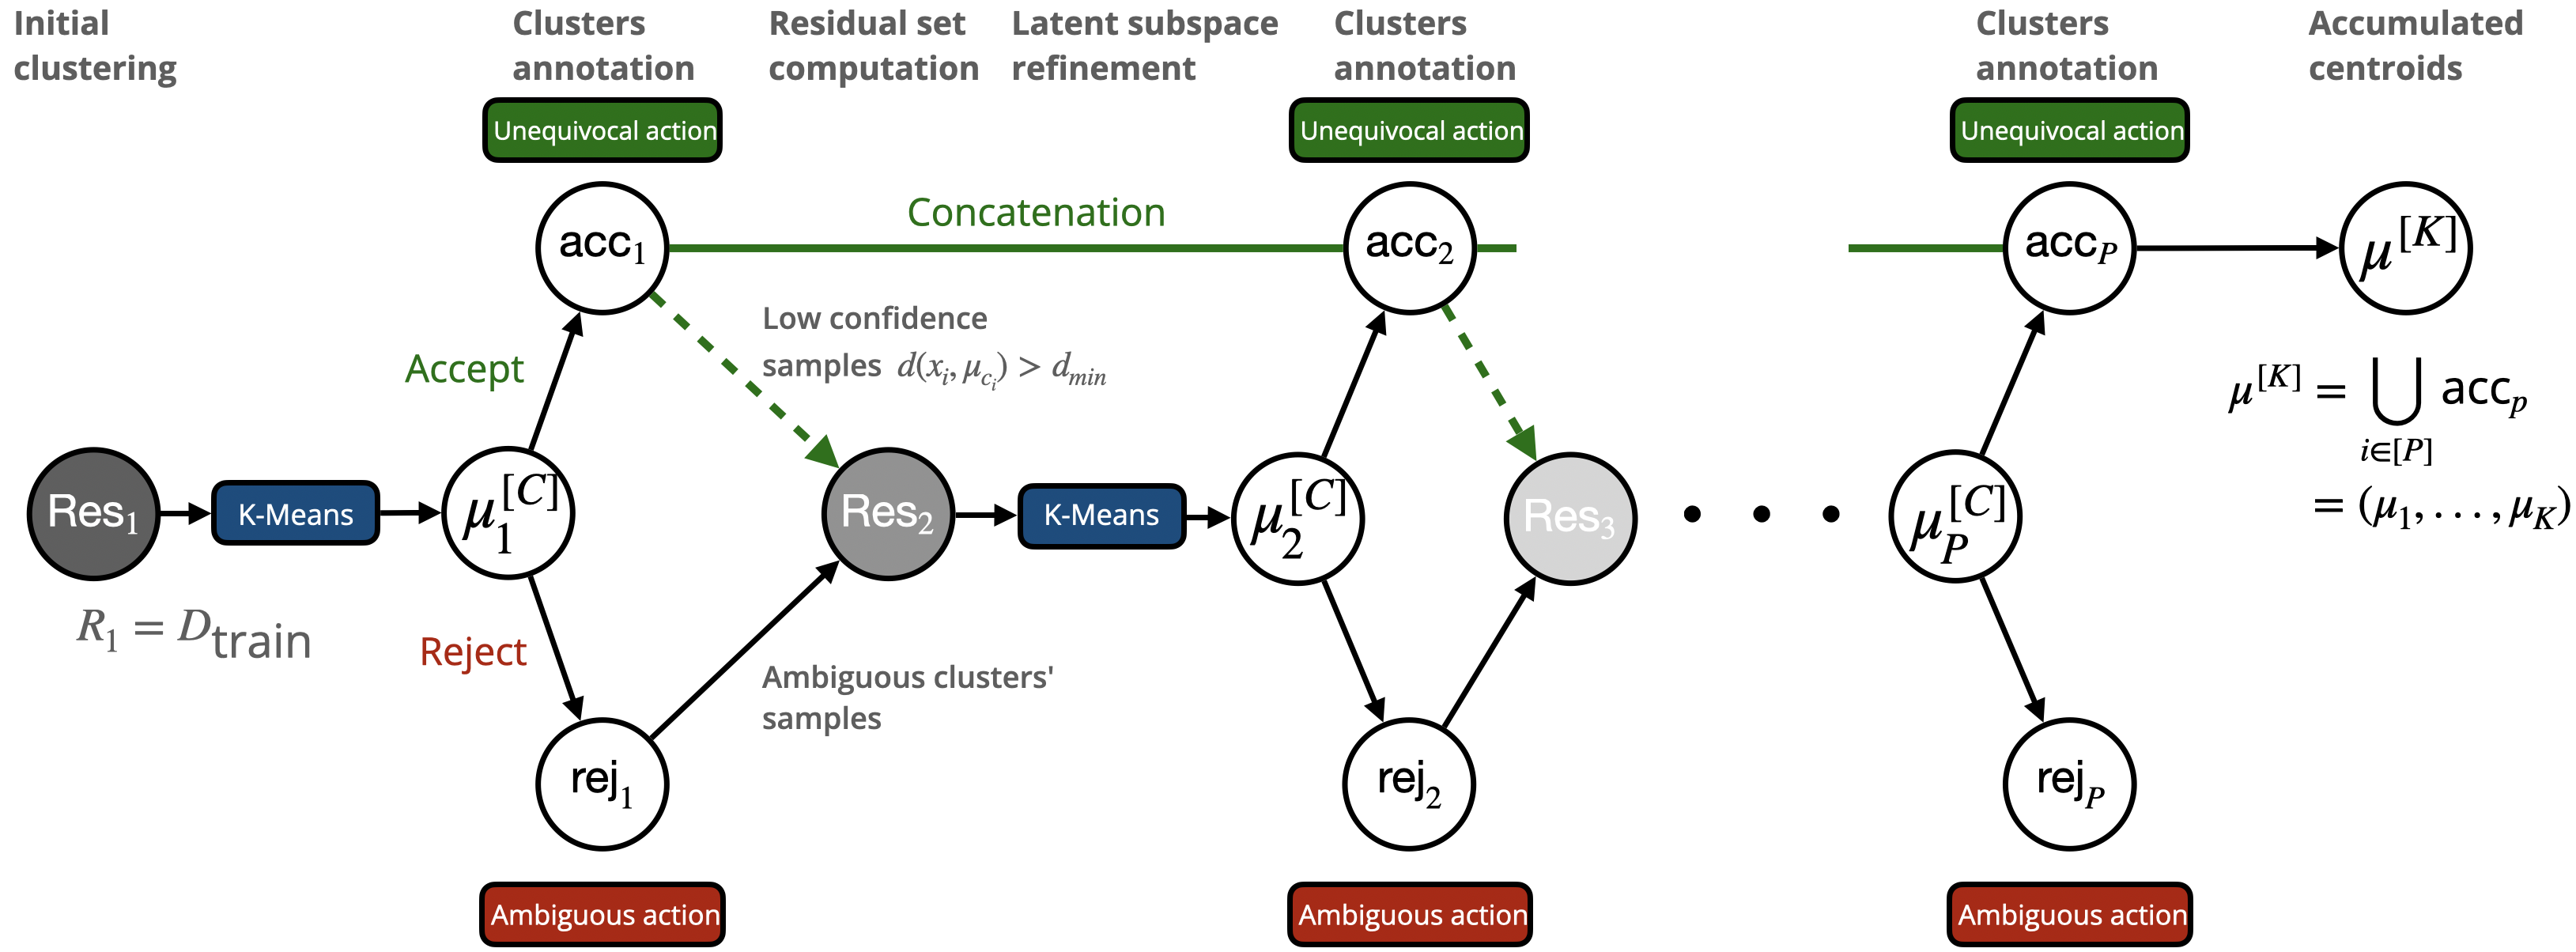
\includegraphics[width = 1.0\linewidth]{figures/chapter_5_recursive_prototypes_workflow_up.png}    
        \caption{\textbf{Illustration of the iterative centroids accumulation step guided by human feedbacks.} Under-segmented regions of the VideoMAE-v2 latent space are iteratively refined to extract fine-grained cluster centroids validated by human annotation. acc$_p$: accepted set of centroids; rej$_p$: rejected set of centroids; Res$_p$: Residual sets}
        \label{fig:chapter_5_recursive_prototypes_workflow}
    \end{figure}

    \subsubsection{Annotation protocol for egocentric vision prototypes.}
    \label{sec:chapter_5_annotation}

    To assess the semantic interpretability of the learned clusters, we introduce a \emph{Visual Probing Mechanism} (VPM) to identify semantically consistent clusters and filter out ambiguous ones.
    At each iteration $p$, the $C$ candidate centroids $\{\mu^p_c\}_{c=1}^C$ are obtained by $k$-means, minimizing within-cluster cosine distance. For each sample $x_i$, we compute its assignment distance to the centroid of its assigned cluster, $d(x_i,\mu^p_{c_i})$, where $c_i=\arg\min_{c\in[C]} d(x_i,\mu^p_c)$. These distances are used to rank samples within each cluster.

    Our VPM relies on the following principles: (i) cluster semantics can be inferred from samples closest to the centroid; (ii) within-cluster semantic consistency can be assessed from the most distant assigned samples; and (iii) the central frame of each input sequence ($\approx 640ms$) is sufficient for visual inspection. In practice, inspecting the nearest and furthest samples from 30 participants per cluster was sufficient for reliable annotation. Representative examples of annotation probes are shown in \Cref{fig:chapter_5_annotation_signal}-a, and detailed validation of these hypothesis are reported in SM~\S4.

    During annotation, clusters whose nearest neighbors exhibit consistent visual patterns corresponding to a single action are accepted, while clusters with heterogeneous semantics are rejected for further refinement. Furthest-neighbor probes typically exhibit weaker semantic alignment, and serve as a quality control by providing a qualitative estimate of assignment errors. As the procedure progresses, furthest neighbors exhibit increased homogeneity and stronger semantic alignment with nearest samples, indicating improved cluster-level semantic consistency, as illustrated in \Cref{fig:chapter_5_annotation_signal}-b. Additional examples of accepted and rejected clusters are presented in SM~\S4.

    Lastly, the annotation step enables practitioners to assign application-relevant labels to the clusters. In our clinical setting, each accepted centroid is classified as \emph{task-related} or \emph{exogenous} to support downstream behavioral analyses, as described in \Cref{sec:downstream_application}.


    \begin{figure}[ht]
        \centering
        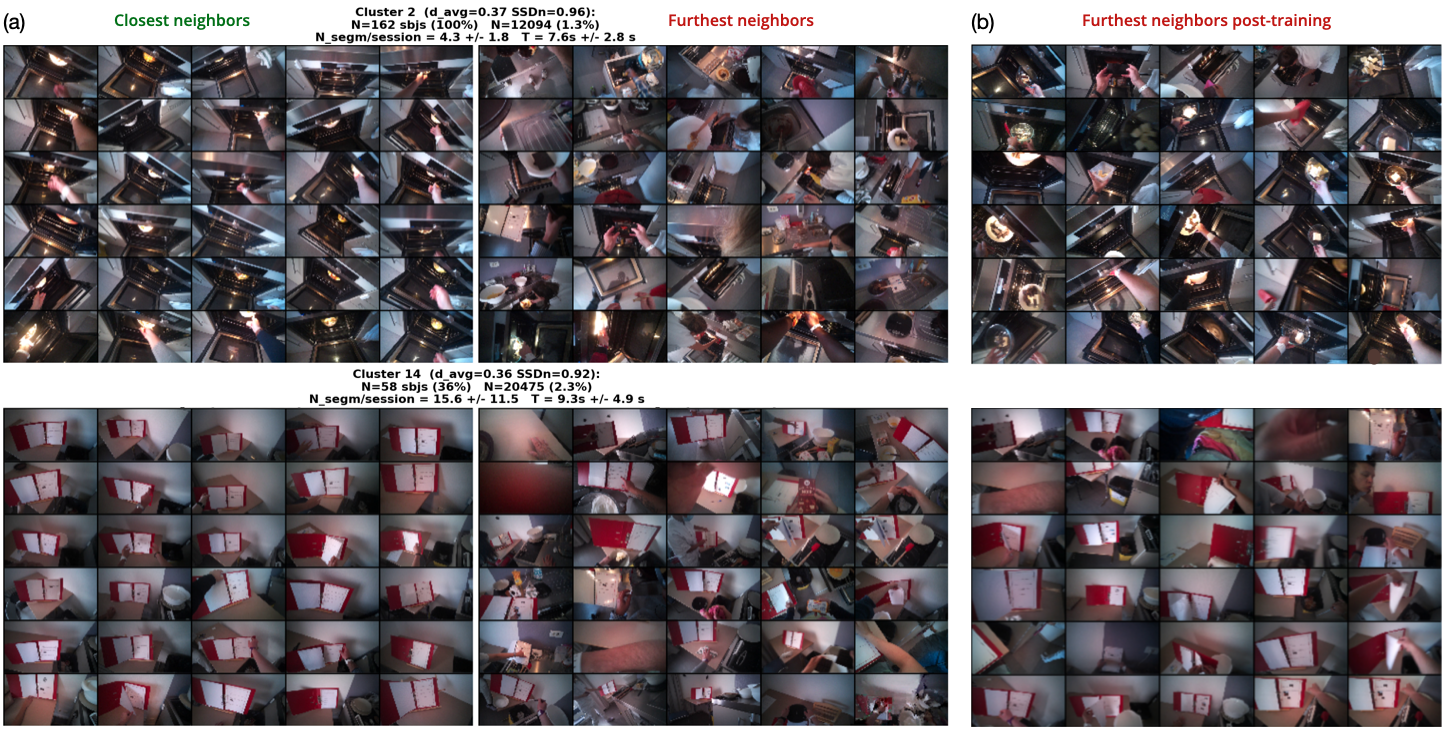
\includegraphics[width = 0.9\linewidth]{figures/chapter_5_annotation_signal_short.png}    
        \caption{\textbf{(a) Two illustrative examples of accepted centroids annotation images, and (b) furthest assigned samples after model training.} We add for each cluster their average assignment distance ($d\_avg$); the normalized sum-of-squared cosine distance (SSDn); the prevalence across subjects and embeddings (N); the average (s.t.d) number of segments occurrences across participants ($N\_segm/session$); and the average (s.t.d.) segments duration across participants (T).}
        \label{fig:chapter_5_annotation_signal}
    \end{figure}


    \subsubsection{Vocabulary consolidation via hierarchical clustering.}

        The accumulation of centroids introduces semantic redundancy, where multiple clusters correspond to the same underlying concept under varying visual conditions. To promote sparsity of the final vocabulary, the accumulated centroids are subsequently consolidated via hierarchical agglomerative clustering (HAC), which defines a reduction mapping $\Phi$ from centroids to prototypes.  The prototypes vocabulary size \(G\) is selected by maximizing the average silhouette score over dendrogram cuts, computed using cosine distance between centroids. In particular, we show in \Cref{fig:chapter_5_silhouette_score}-a that HAC outperforms alternatives such as K-means, DBSCAN/HDBSCAN, GMMs, and spectral clustering. In practice, two consecutive consolidation stages are applied to address residual redundancy: the first stage groups similar centroids, while the second stage uses mean-aggregate representations within each prototype to further consolidate near-duplicate clusters (see \Cref{fig:chapter_5_silhouette_score}-(b,d)). 
            
        \begin{figure}[ht]
                \centering
                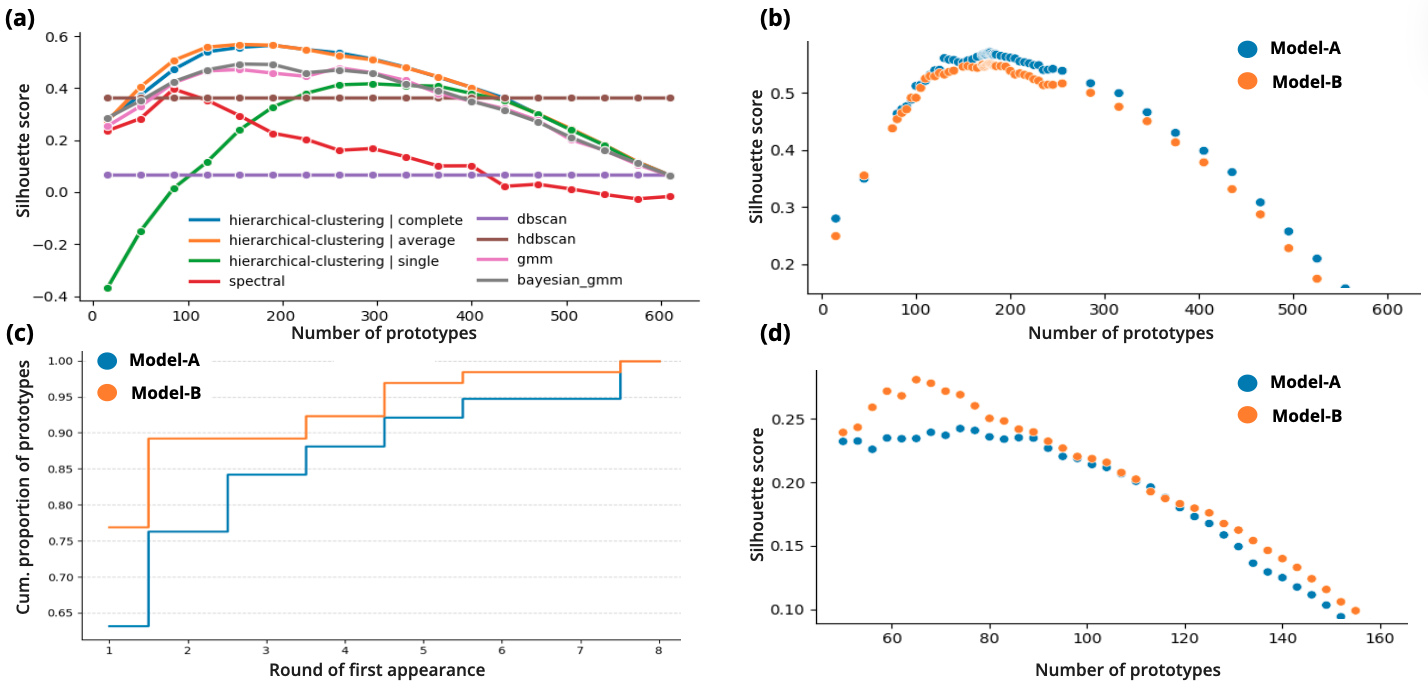
\includegraphics[width=0.9\linewidth]{figures/pannel_ss.png}    
                \caption{\textbf{Evolution of the silhouette score across number of estimated prototypes (a) across clustering methods, (b) during the $1^{st}$ and $2^{nd}$ (d) consolidation stages. (c) Cumulative proportion of final prototypes per round of appearance.}}
                \label{fig:chapter_5_silhouette_score}
            \end{figure}

    \subsection{Unsupervised temporal action segmentation}
        \label{sec:chapter_5_unsupervised_temporal_segmentation}

        To leverage temporal structure, we perform unsupervised temporal action segmentation independently for each participant. Given embeddings $X = (x_1,\dots,x_n)$, the goal is to partition the sequence into contiguous segments corresponding to semantically consistent actions. We use kernel-based change-point detection (KCP)~\cite{cpt,garreau2018consistent}, which detects mean-shifts in a Reproducing Kernel Hilbert Space (RKHS), focusing on action boundaries rather than classes.

        \paragraph{Kernel-based change-point detection.}

        Let $k(\cdot,\cdot)$ be a positive semidefinite kernel applied to latent embeddings. KCP reformulates change-point detection as a segmentation problem in the associated RKHS, where each segment is approximated by its empirical mean \cite{4301363,cpt,garreau2018consistent}. For a candidate segmentation $\tau = \{0=t_0 < \dots < t_M=n\}$ with $M$ segments, we minimize the penalized empirical risk
        \begin{equation}
        \label{eq:opti}
        \hat{\mathcal{R}}_{n,\lambda}(\tau)
        =
        \frac{1}{n} \sum_{m=0}^{M-1} \sum_{i=t_m}^{t_{m+1}-1}
        \big\| \phi(x_i) - \bar{\mu}_{t_m:t_{m+1}} \big\|_{\mathcal{H}}^2
        + \frac{\lambda}{n} M,
        \end{equation}

        where $\phi: \mathbb{R}^D \to \mathcal{H}$ is the implicit feature map induced by $k$, $\bar{\mu}_{t_m:t_{m+1}}$ denotes the empirical RKHS mean of segment $m$, and the regularization hyperparameter $\lambda$ controls the number of change points. The optimization is solved exactly using the pruned exact linear time (PELT) algorithm~\cite{pelt}, yielding an efficient nonparametric procedure that does not require specifying the number of segments in advance. The detailed optimization procedure to solve \Cref{eq:opti} using dynamic programming can be found in \cite{cpt}, and is implemented efficiently in the \texttt{ruptures} package \cite{ruptures}. 

        \paragraph{Penalty calibration.} Following \cite{cpt,CELISSE2018200,slop_heuristics_survey}, we select the penalty parameter using the slope heuristic, which identifies the optimal regularization by detecting a characteristic slope change in the model complexity versus penalty curve. We ensure comparability across participants by estimating a single shared penalty using a fixed-effect formulation rather than tuning $\lambda$ independently for each sequence.
    \vspace{-0.2cm}
    \subsection{Symbolic representation}
        \label{sec:chapter_5_symbolic_representation}

        The final symbolic representation combines the consolidated prototype vocabulary $\mathcal{V}$ with participant-specific temporal segmentations. Given a latent embedding sequence $\mathbf{X} = (x_1, \ldots, x_n)$, each sample is assigned to its nearest centroid and mapped to a prototype via the reduction mapping $\Phi$. Each embedding $x_i$ is then assigned to its closest centroid $\mu_k$ under cosine distance, yielding a prototype label $y_i = \Phi(\arg\min_k d(x_i, \mu_k))$. To reduce assignment noise, we filter unreliable assignments using a prototype-specific threshold: for each prototype $g$, we compute the mean $m_g$ and standard deviation $\sigma_g$ of their empirical assignment distances, and reject assignments exceeding $m_g + \sigma_g$ by assigning them to a background label ($\tilde{y}_i = -1$).

        \paragraph{Segment-level label aggregation.} Given a temporal segmentation $\tau = (t_0, \ldots, t_M)$ and filtered labels $\tilde{\mathbf{y}}$, we assign a single label to each segment via majority voting over its central half (excluding boundary frames prone to unstable assignments):
        \[
        s_j = \operatorname{MajVote}\{\tilde{y}_i : i \in [t_{j-1}+\tfrac{\ell_j}{4},\; t_j-\tfrac{\ell_j}{4}]\},
        \quad \ell_j = t_j - t_{j-1}.
        \]
        The final symbolic sequence assigns $s_j$ to all indices within segment $j$. Lastly, short segments (fewer than four embeddings, i.e., $\approx 1.2s$) flanked by identical labels are merged, yielding a piecewise-constant representation.

\vspace{-0.2cm}
\section{Experimental setting}
    \label{sec:experimental_setting}

    \subsection{Dataset}

    Data were collected from 162 administrations of a standardized cooking task in a controlled environment, consisting of following the instructions of a recipe to bake a chocolate cake \cite{Chevignard2008}. These sessions correspond to $N=122$ unique participants: 26 healthy controls and 96 patients with dysexecutive syndromes. Egocentric videos were recorded using an eye-tracker camera at 25\,fps. Task durations ranged from 15 to 90 minutes (median: 32 min), yielding 905,903 embeddings in total.
    \vspace{-0.1cm}
    \subsection{Model estimation}

    Sessions are split at the subject level into training (80\%, 129 sessions from 98 participants, 725,335 embeddings) and test (20\%, 33 sessions from 24 participants, 180,568 embeddings) sets to assess generalization. To evaluate robustness to annotator subjectivity, two independent vocabularies (\texttt{Model-A} and \texttt{Model-B}) are estimated using feedback from different annotators. Centroids are collected over $P=8$ rounds with $C=100$ centroids per round---the maximum that did not degrade clustering quality given the training sample size---yielding $K_{\text{in}}=800$ centroids prior to consolidation, chosen to exceed significantly the average number of detected action segments ($\bar{M}=274$, STD$=24$). The final vocabulary size is determined by HAC consolidation. Cosine $k$-means is implemented via the \texttt{Faiss} library \cite{douze2024faiss}, which outperformed alternatives in preliminary experiments.
\vspace{-0.2cm}
\section{Evaluation protocol and results}
\label{sec:chapter_5_evaluation_protocol}

    In the absence of ground-truth action labels, we adopt a multi-level evaluation protocol designed to assess: 
    (i) the semantic consistency of the learned prototypes, 
    (ii) the robustness of the symbolization procedure to subjective human feedback, and (iii) the fidelity and generalizability of prototypes assignments to empirical samples, in particular across unseen particants.

    \subsection{Prototyping outcomes and semantic validity}

    Since consolidation may merge visually distinct actions, we evaluate prototype validity through systematic visual inspection. For each prototype, a visual probe is constructed by aggregating the probes of its constituent centroids (SM~\S4.4). Prototypes are retained if all constituent centroids encode a single, unambiguous action. 

    \paragraph{Results.} After eight centroid-collection rounds ($K_{\text{in}}=800$), annotators retained $\approx 80\%$ of centroids ($642$ and $613$ for \texttt{Model-A} and \texttt{Model-B}). While the majority of final prototypes emerge from the first iteration, subsequent rounds contribute additional semantically distinct actions, demonstrating that the iterative procedure effectively discovers novel prototypes (\Cref{fig:chapter_5_silhouette_score}-(c)). Two successive HAC consolidation stages reduced these to $G=75$ and $G=65$ final prototypes (detailed progression in SM~\S5). Of the consolidated prototypes, $55$ ($73.3\%$) and $45$ ($69.2\%$) were validated as capturing unique actions---rejections mainly resulted from merges of visually similar but semantically distinct actions. Qualitatively, the discovered prototypes span the full range of task-relevant actions (e.g., recipe reading, ingredient manipulation, oven operation) as well as exogenous behaviors (e.g., looking around the room, examiner interactions), without requiring predefined action categories. In the remainder of the evaluation, only validated prototypes are considered.

    \subsection{Sensitivity to human feedback subjectivity}

    We compare \texttt{Model-A} and \texttt{Model-B} at three levels: (i) inter-rater reliability on a shared annotation set measured using Cohen's $\kappa$ coefficient \citep{cohen1960}, (ii) vocabulary-level semantic comparison using embedding co-occurrence Hungarian matching, and (iii) agreement between downstream symbolic representations using Normalized Mutual Information (NMI) and Adjusted Rand Index (ARI).

    \paragraph{Results.} On $n=400$ shared images, annotators exhibited moderate agreement on ambiguity judgments (Cohen's $\kappa=0.44$, 95\% CI: $[0.35, 0.54]$) but substantial agreement on the task/exogenous distinction ($\kappa=0.78$, 95\% CI: $[0.57, 0.93]$), indicating variability stems from subjective ambiguity rather than semantic disagreement. Importantly, both vocabularies capture the same range of actions: prototype matching reveals one-to-one correspondences with no action missing from either model. Downstream symbolic representations show strong agreement (NMI$=0.791$, 95\% CI: $[0.790, 0.792]$; ARI$=0.682$, 95\% CI: $[0.680, 0.685]$) and nearly identical temporal granularity: median durations $6.4$s vs.\ $6.6$s, segment counts $1{,}247\pm290$ vs.\ $1{,}298\pm310$. Additional details and visualizations are provided in SM~\S7--8.

    \subsection{Fidelity and generalizability of symbolic representations}

    In the absence of ground-truth labels, we evaluate fidelity and generalizability through visual probing: (i) generalizability is assessed by comparing nearest-neighbor probes between training and held-out participants, (ii) fidelity is probed by inspecting furthest-neighbor samples of each prototype to test if distant assignments preserve semantic consistency, and (iii) coverage is assessed qualitatively via both UMAP projection of prototypes' centroids against empirical samples and visual inspections of the furthest-neighbors.

    \paragraph{Results.} The estimated prototypes transfer well to held-out participants: nearest-neighbor visual probes revealed highly stable visual semantics between training and test subjects. This is corroborated by the overlap between UMAP projections of both training and testing samples, presented in SM~\S6. We note that this strong generalizability can be theoretically attributable to the \textit{prescribed} nature of the task, performed in a reproducible setting, and the consistent use of the same head-mounted camera and video encoder. Furthest-neighbor samples preserved prototype semantics, validating the distance-based filtering heuristic and ensuring the accuracy of the symbolic representations. However, visually similar actions (e.g., pouring different ingredients) were not consistently disentangled at the centroid level, reflecting both the limited discriminative power of the video encoder and the need for refined residual space definitions in the iterative procedure.

    % Background label assignments are also largely consistent across models ($80\%$ non-background, $12\%$ background, $8\%$ discrepancy), suggesting that background detection reflects genuine uncertainty rather than instability of the symbolization process (full comparison metrics and temporal granularity analysis in SM~\S9).

    Taken together, these results demonstrate that the proposed symbolization procedure yields fine-grained and temporally accurate proxy representations of participants' behavior, capturing a broad range of actions with strong generalizability to unseen participants. Independent annotators produced vocabularies that, despite minor subjective differences in centroid selection, exhibited strong semantic alignment and temporal consistency---validating their use for downstream behavioral analysis.


\section{Application of the symbolic representations to the characterization of behavioral manifestations associated with dysexecutive syndromes}
    \label{sec:downstream_application}

    We demonstrate the clinical utility of the symbolic representations by analyzing behavioral differences across diagnosis groups: 26 healthy controls, 59 patients with traumatic brain injury (TBI), and 37 with radiation-induced leukoencephalopathy (RIL), associated with more severe executive impairment. All analyses use the \texttt{Model-A} vocabulary, combining validated prototypes with original centroids when consolidation introduced ambiguity, yielding $G=150$ prototypes manually grouped into 28 action categories (\Cref{fig:chapter_6_vocabulary_SR}-a).


    \begin{figure}[ht]
        \centering
        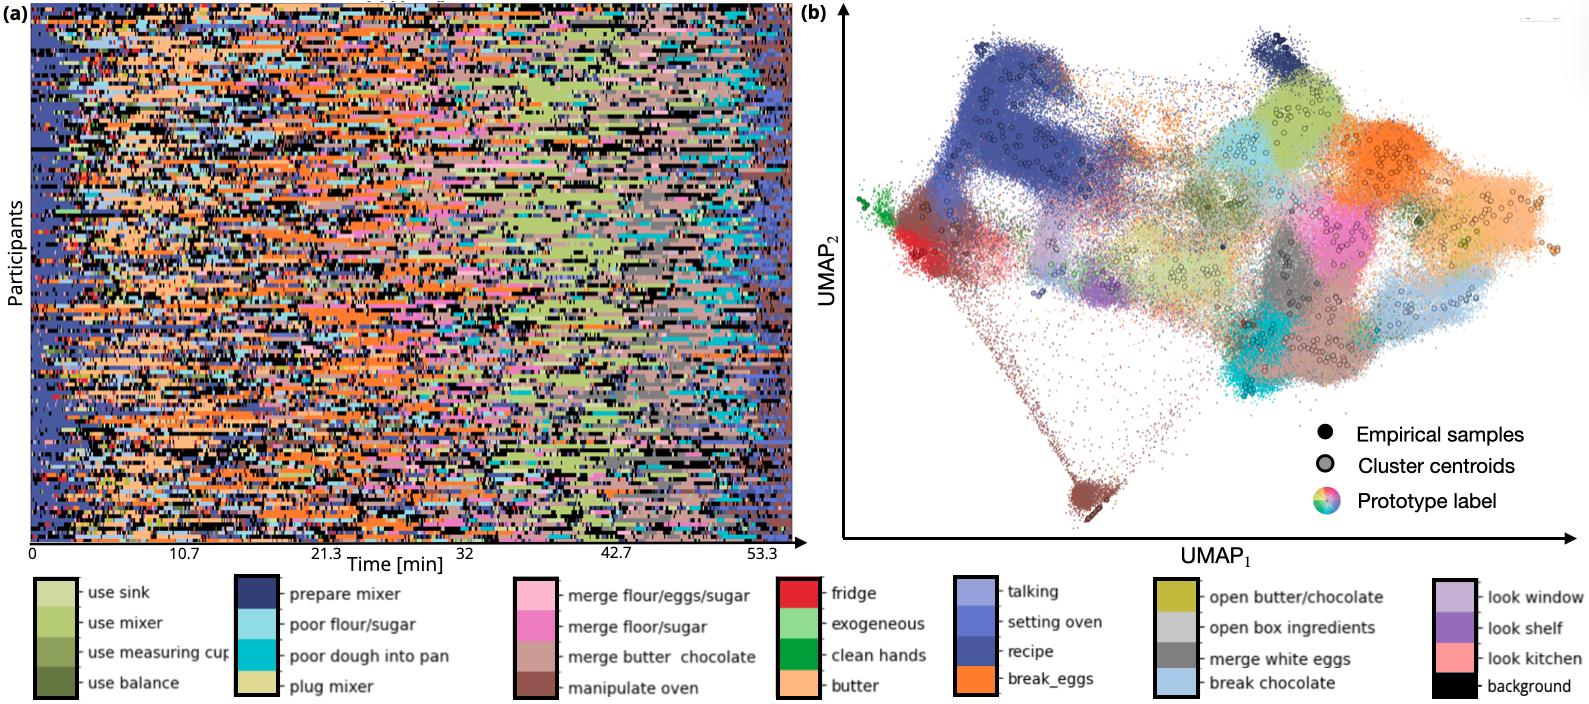
\includegraphics[width = 1.0\linewidth]{figures/pannel_results_short.png}    
        \caption{\textbf{(a) Symbolic representations of participants' egocentric vision during the procedural task, and (b) two-dimensional UMAP projection of training samples and prototype centroids.} Each row in (a) corresponds to a participant, with colors indicating prototype assignments (sequences upsampled for visualization).}
        \label{fig:chapter_6_vocabulary_SR}
    \end{figure}

    \subsection{Temporal organization}

    Task fragmentation, quantified as symbolic segments per unit time, differed significantly across groups (likelihood-ratio test $\chi^2(2)=11.53$, $p=3.31\times10^{-3}$). Participants with RIL exhibited $22.9\%$ longer segment durations than controls, while those with TBI showed $8.1\%$ longer durations. These findings align with recent reports linking reduced activity fragmentation to cognitive impairment \cite{10.1001/jamanetworkopen.2021.35168,Khosla2025}. Statistical details are provided in SM~\S9.

    \subsection{Action composition across diagnosis groups}

    We analyzed group differences in action composition by computing, for each of the 28 categories: number of occurrences, mean duration, and proportion of task time. Pairwise group comparisons were performed using Mann-Whitney U tests with rank-biserial correlation ($r_{rb}$) as effect size, and Benjamini-Hochberg correction for multiple comparisons. Two key patterns emerged (SM~\S9).

    \paragraph{Task-related vs.\ exogenous actions.} Participants with RIL spent a significantly higher proportion of time on exogenous actions (e.g., looking around the room, talking to the examiner) compared to both controls ($p=8.15\times10^{-3}$, median $17\%$ vs.\ $8.3\%$) and TBI patients ($p=2.18\times10^{-3}$, median $17\%$ vs.\ $9.1\%$). No significant difference was found between TBI and controls. This pattern is consistent with known deficits in sustained attention and goal-directed behavior in severe dysexecutive syndromes \cite{Hendry2016sh}.

    \paragraph{Category-specific findings.} Severity of executive impairment was associated with increased recipe consultations (RIL vs.\ Control: $p_{\text{corr}}=3.8\times10^{-3}$, $r_{rb}=0.65$; TBI vs.\ Control: $p_{\text{corr}}=0.015$) and reduced time spent on core task actions such as merging the dough (RIL vs.\ Control: $p_{\text{corr}}=2.3\times10^{-3}$, $r_{rb}=-0.68$). These findings corroborate impairments in prospective and episodic memory leading to failures to remember instructions \cite{Hendry2016sh,Chevignard2008}. Participants with RIL also exhibited longer oven manipulation durations ($p_{\text{corr}}=0.014$, $r_{rb}=0.61$) and more frequent examiner interactions compared to TBI patients ($p_{\text{corr}}=8.2\times10^{-3}$, $r_{rb}=-0.46$). Notably, examiner interactions are part of the standardized error categories counted by neurologists during this ecological assessment~\cite{Chevignard2008}, suggesting that the symbolic representations recover clinically relevant behavioral markers. The complete per-category analysis is provided in SM~\S10.

    %Taken together, these results demonstrate that the proposed symbolization procedure yields fine-grained and temporally accurate proxy representations of participants' behavior, capturing a broad range of actions with strong generalizability to unseen participants. Independent annotators produced vocabularies that, despite minor subjective differences in centroid selection, exhibited strong semantic alignment and temporal consistency---validating their use for downstream behavioral analysis.

\section{Discussion}
    \label{sec:chapter_5_conclusion}

    We presented a framework for constructing interpretable symbolic representations of egocentric video by combining a pretrained video encoder with iterative human-in-the-loop prototype refinement. Unlike pose-based behavioral representations that operate on body coordinates, the prototype explicitly encode rich egocentric visual experience that is crucial to understanding goal-directed behavior. While human feedback guides the rejection of ambiguous clusters, the definition of action categories remains fully unsupervised, and independent annotators produced semantically aligned vocabularies with consistent downstream representations. Importantly, this approach drastically reduces annotation effort compared to exhaustive frame-level or segment-level labeling: annotators provide simple binary accept/reject decisions on candidate cluster probes ($\approx$1-15s per cluster and $\approx$1-60s per prototype), replacing hours of manual video annotation with minutes of visual inspection. The recursive procedure including clustering, visual probes generation, and annotations can be applied entirely (P=8) within a single day on a standard server\footnote{We used for the experiments a dual-socket Intel Xeon Gold 5220R system (48 cores, 256 GB RAM)}, making the approach computationally efficient and practical for large-scale behavioral studies.

    The learned prototypes generalize well to held-out participants, a property we attribute to the prescribed nature of the task, reproducible acquisition conditions, and the use of a shared encoder. This suggests that the approach could extend to other standardized procedural tasks where visual regularities are expected; however, validation on multi-environment benchmarks remains an open direction, as existing large-scale egocentric datasets typically lack the single-environment characteristic that enables cross-participant prototype transfer. A current limitation lies in the consolidation stage: similarity-based hierarchical clustering may merge visually close but semantically distinct actions, requiring manual inspection to preserve vocabulary integrity. Integrating temporal dynamics or object-level cues into consolidation could reduce this ambiguity.

    Beyond enabling scalable behavioral comparisons without dense action labeling, the symbolic representations provide a principled anchor for multimodal integration: complementary signals such as gaze patterns, pupillometry, or speech can be analyzed within specific action contexts, while temporally aligned modalities could enrich the characterization of action segments themselves.

% \subsubsection{Acknowledgements} Please place your acknowledgments at
% the end of the paper, preceded by an unnumbered run-in heading (i.e.
% 3rd-level heading).


% ---- Bibliography ----
% BibTeX users should specify bibliography style 'splncs04'.
% References will then be sorted and formatted in the correct style.
\bibliographystyle{splncs04}
%\bibliographystyle{ieeetr}
\bibliography{bibliography}


\end{document}